\subsection{Iteration 4}

The focus of iteration 4 was a summative test.

First, a pre-test was carried out in paper, including questions about the coach and an entrepreneurship quiz, based on a well-known study \citep{general-entrepreneurship-quiz}, see Appendix \ref{pre-test}.

During the test, this was the first time that the app could send data to the server. Data was sent whenever a quiz was started, and whenever a quiz was finished.

The group was divided into two, the ones who brought manuals and they who did not. Those that had brought manuals, could use these with the app, see figure \ref{fig:appevaluation}.

\begin{figure}[h]
    \centering
    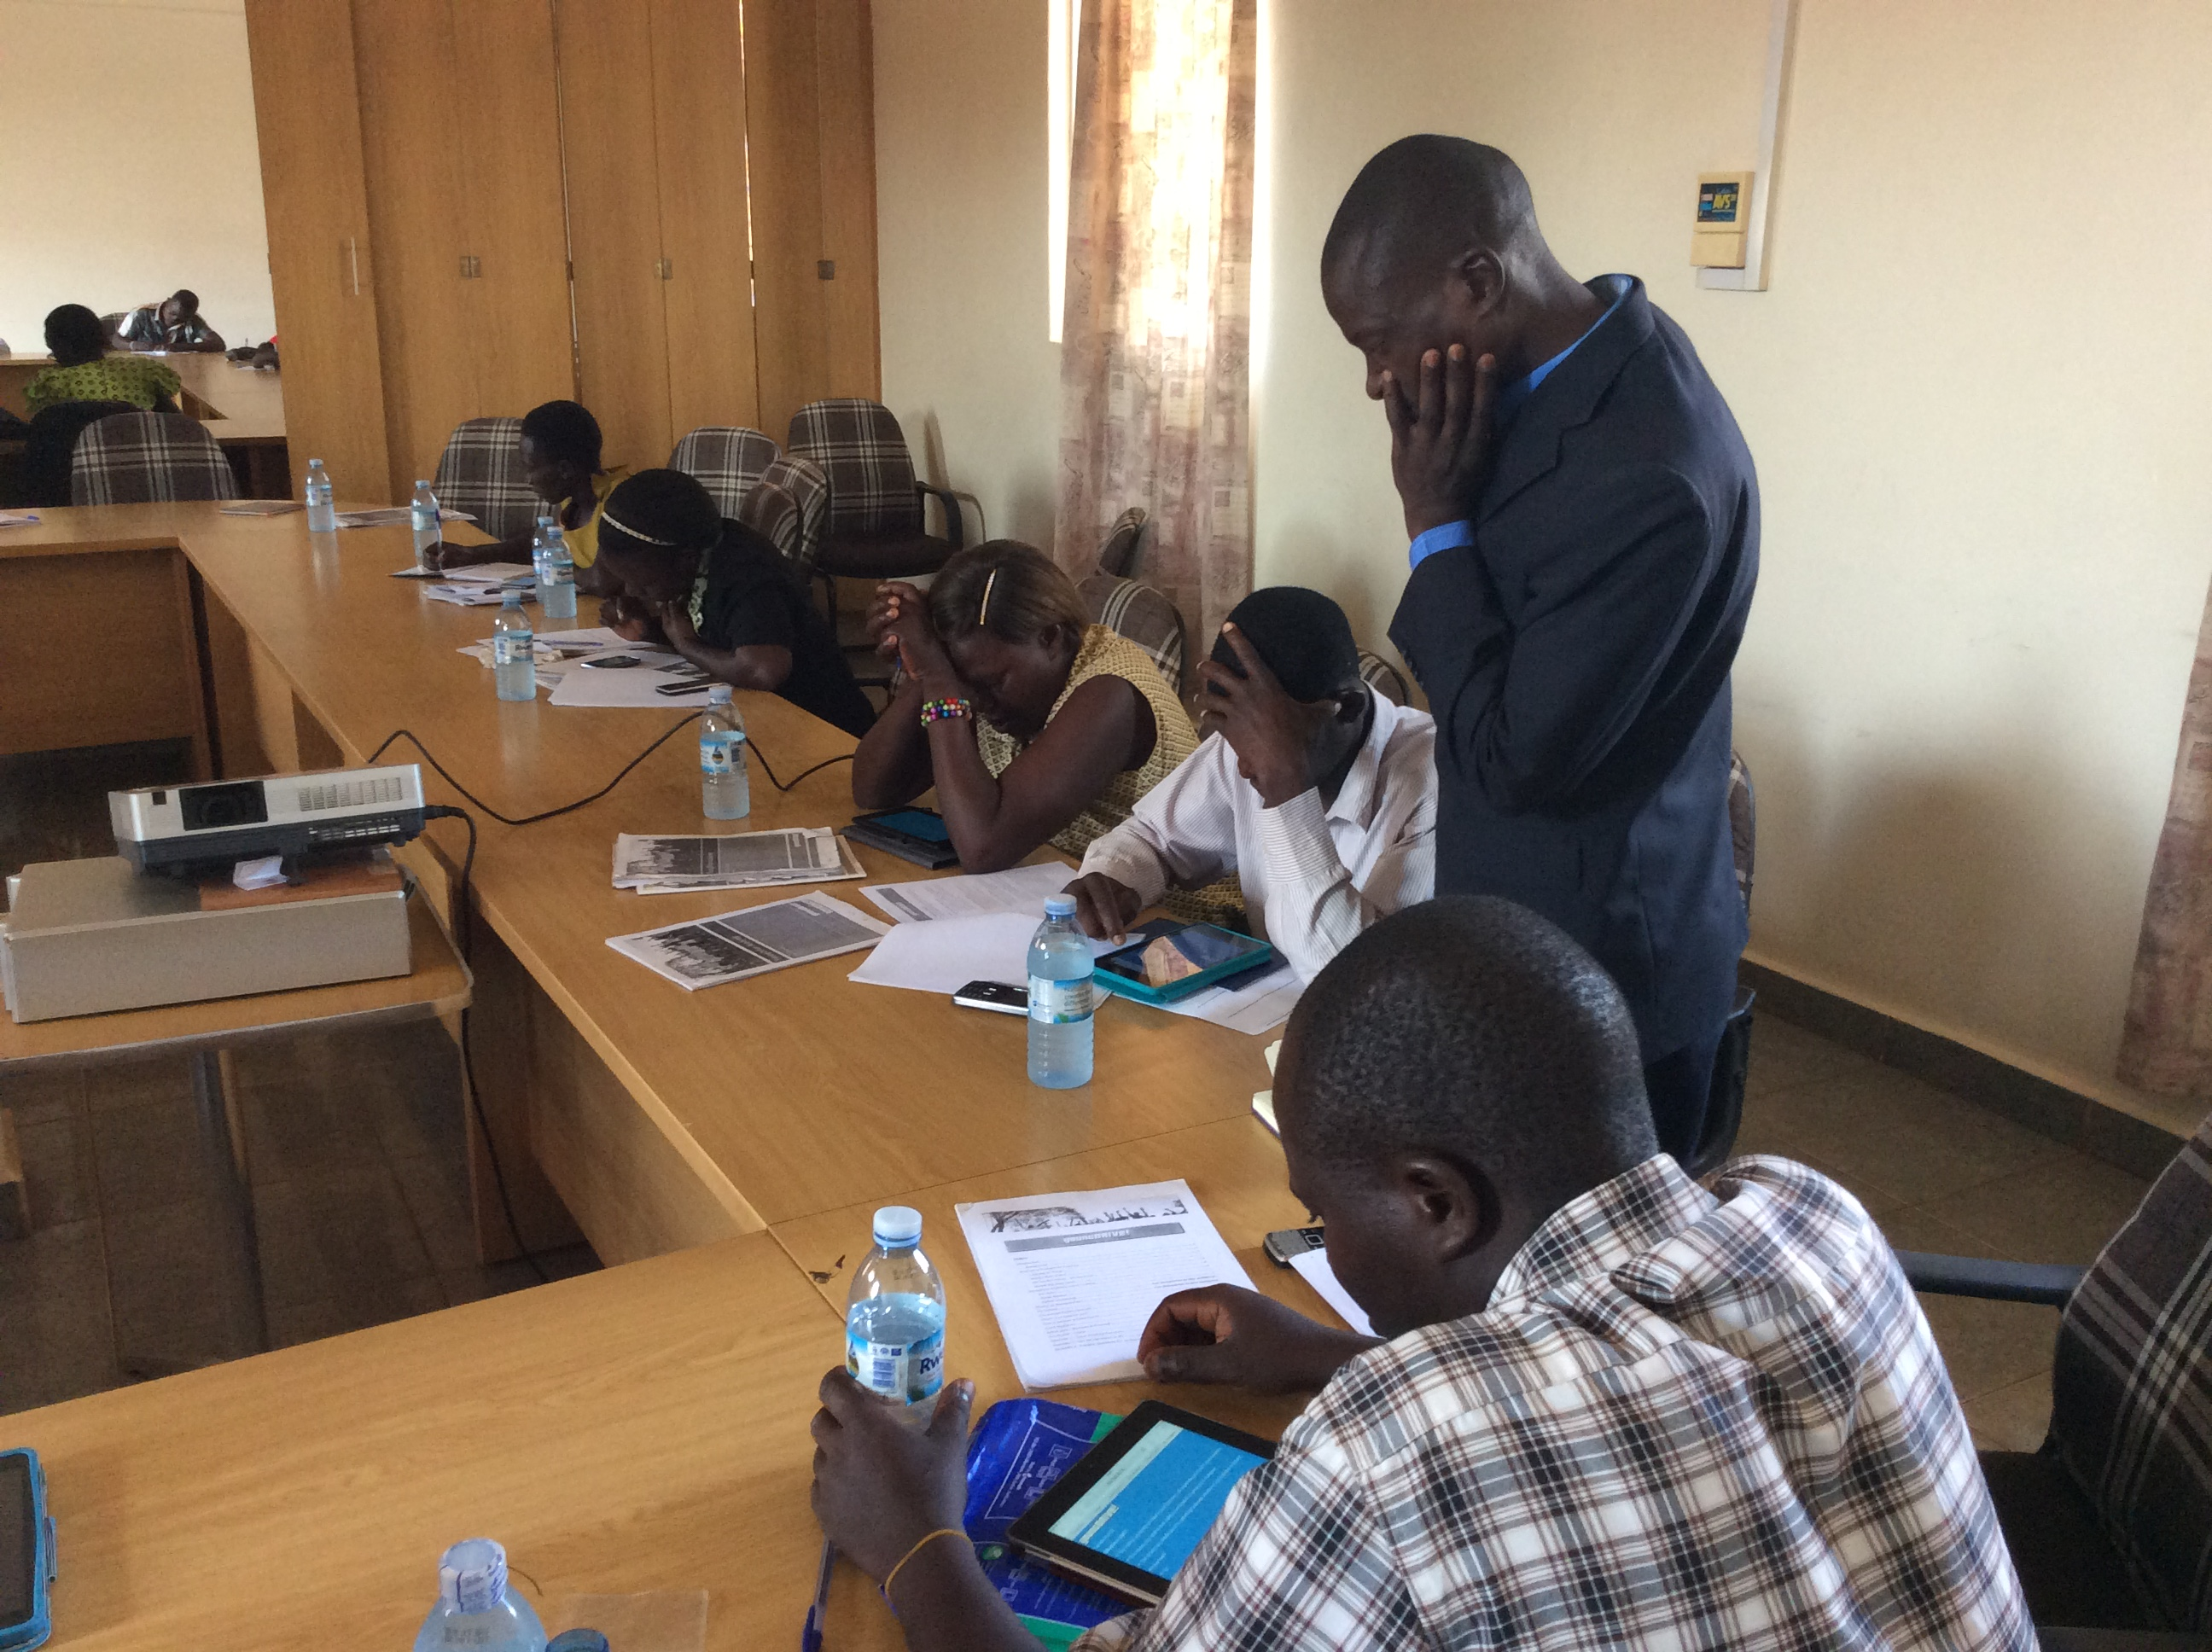
\includegraphics[width=0.7\textwidth]{appevaluation.jpg}
    \caption{Coaches answering the app questions for topic quiz 3 on Financial Literacy, and the coach guide quiz 9 on Action Plan.}
    \label{fig:appevaluation}
\end{figure}

After the test, every coach was divided into one or three groups, on random. In these groups, they were asked:

\begin{enumerate}
\item Why do you think you were correct or incorrect?
\item Do they like the app?
\item Are you stimulated by the app?
\item What did you like?
\item What did you not like?
\item When do you want to use the app?
\item When are you not able to use the app?
\end{enumerate}

To analyse the paper-submitted data, all of this was combined first into a Google Spreadsheet. (The app results were also recorded in paper, but only as a backup.) Data collection was done by the app itself, which pushes data to server whenever online (it saves quiz start, and quiz finish).

The next day, a small app evaluation and co-creation workshop was held for the Educator Dashboard, and the final version of the app. Also, a test was done with the Plan Tororo staff.

Back in Kampala, a presentation was held with Plan International. Back in Sweden, a presentation was held with the YoungDrive Strategic Management Team.
